\documentclass[12pt]{article}
\usepackage[pdftex]{color, graphicx}
\usepackage{amsmath, amsfonts, amssymb, mathrsfs}
\usepackage{dcolumn}
\usepackage{natbib}
\usepackage{wrapfig}
\usepackage{subfig}
\usepackage{float}
\bibpunct{(}{)}{;}{a}{}{,}

\oddsidemargin=0.25in
\evensidemargin=0.25in
\textwidth=6in
\textheight=8.75in
\topmargin=-.5in
\footskip=0.5in


%\date{due Sep 17th}

\title{Homework6}



\begin{document}

%\maketitle
\newcommand{\argmin}{\text{argmin}}

\noindent STAT5014\\
 Homework 6\\
 Due Oct.8th

\begin{center}
\noindent
\section*{Confidence Interval for the Probability of Success for the Bernoulli Probability Distribution} %this is a comment
\noindent Yin Yuan\\

\vspace{.25 in}
\end{center}

\subsection*{Brief Introduction}

This homework aims to verify whether the "empirical" coverage probability of CI based on Wald's approximation using Monte Carlo simulation is comparable to the theoretical coverage probability of CI. The CI can be interpreted as the ratio of times that the CI can cover the real parameter value in the experiments, i.e., for a 90\% CI, it will cover the real parameter value 90 out of 100 times if we repeat the experiment 100 times. We can construct our algorithm based on theinterpretation of CI.




\subsection*{Method}

We first simulate random numbers from the Bernoulli distribution with different "$p$" values; then we compute the CI for different "$p$" based on the simulated samples using the symmetric Wald interval algorithm; we count the number of times $n$ that "$p$" covered by the estimated CI by repeat the previous steps 1000 times; finally we compute teh "empirical" coverage probability for different "p" as $n/1000$.

\subsection*{Result and Conclusion}

The CI coverage probability result using simulated samples is illustrated in Fig.~\ref{fig:img1}. We can see that for "$p$" close to 0 and 1 have lower real coverage probability however for most of the "$p$"s, the real coverage probability is oscillating between 90\%, which means that the estimated "empirical" coverage probability is a resonable approximation of the real coverage probability.


\begin{figure*}[hptb]
	\centering
{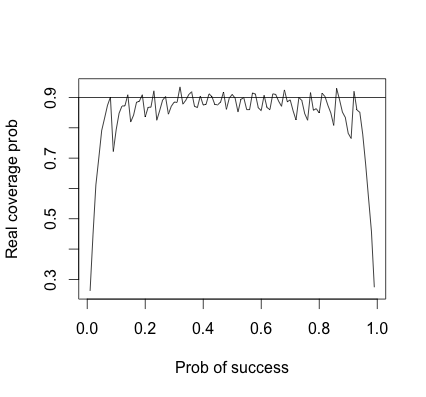
\includegraphics[scale=1]{Rplot01.png}} \;
\caption{CI coverage prob.}
	\label{fig:img1}
\end{figure*}


\subsection*{Appendix: R code}
\begin{verbatim}

P <- c(1:99)/100
N <- 30    
EP <- rep(0, length(1:99)) 
Nt <- 1000 # number of trials for each "P"

# function for compute CI for "p"
binomCI=function(y, p, alpha1, alpha2) {
  z1<-abs(qnorm(alpha1))
  z2<-abs(qnorm(1-alpha2))
  nn<-length(y)
  phat<-sum(y)/nn
  se<-sqrt(phat*(1-phat)/nn)
  return(c(phat-z1*se, phat+z2*se))
}

for (i in 1:length(P)) {
  print(P[i])
  count<-0
  for (times in 1:Nt) {
    # generate random numbers with Bernoulli distribution
    rb<-rbinom(N, 1, P[i])
    # compute CI for "p"
    CI<-binomCI(rb, P[i], 0.05, 0.05)
    # count number of success
    if (CI[1]<=P[i] & CI[2]>=P[i]) {
      count<-count+1
    }
  }
  # record ratio of success
  EP[i]<-count/Nt
}

plot(P, EP, type="l", xlab="Prob of success", ylab="Real coverage prob")
abline(h=0.9)


\end{verbatim}



\end{document}



